\documentclass[11pt]{article}
\usepackage[top=1.00in, bottom=1.0in, left=1in, right=1in]{geometry}
\renewcommand{\baselinestretch}{1.1}
\usepackage{graphicx}
\usepackage{natbib}
\usepackage{amsmath}
\usepackage{gensymb}
\usepackage{xcolor}
\usepackage{xr-hyper}
\externaldocument{bayesianflowsysupp}
\usepackage{lineno}
\newcommand{\R}[1]{\label{}\linelabel{#1}}

\def\labelitemi{--}

\usepackage{fancyhdr}
\pagestyle{fancy}
\fancyhead[LO]{}
\fancyhead[RO]{}

\begin{document}
\bibliographystyle{/Users/Lizzie/Documents/EndnoteRelated/Bibtex/styles/amnat}
\renewcommand{\refname}{\CHead{}}

%%%%%%%
%% To do %%
%%%%%%%
% https://github.com/lizzieinvancouver/gelmanhill/wiki/Vocabulary

\title{A four-step simulation-based workflow for ecological analysis and science}
% Simulation as a best practice in Bayesian workflows and beyond
% How to fit Bayesian models and influence people
% How to do Bayesian model fitting in ecology 
% The best way to be a Bayesian in ecology today
% \date{\today}
\author{EM Wolkovich$^{1*}$, T Jonathan Davies$^{1,2}$, William D Pearse$^{3,4}$ \& Michael Betancourt$^{5}$}
\maketitle

\noindent $^{1}$ Forest and Conservation Sciences, University of British Columbia, Vancouver, BC V6T 1Z4, Canada\\
$^{2}$ Botany, University of British Columbia, Vancouver, BC V6T 1Z4, Canada\\
$^{3}$ Department of Life Sciences, Imperial College London, Ascot SL5 7PY, United Kingdom \\
$^{4}$ Alan Turing Institute, British Library, 96 Euston Road, London NW1 2DB, United Kingdom \\
$^{5}$ Symplectomorphic, LLC, New York, NY 10026, USA \\
$^{*}$ \url{mailto: e.wolkovich@ubc.ca}
 
\vspace{3ex}
\noindent \emph{Keywords:} big data; scientific workflow; data simulation; prediction; null hypothesis testing, machine learning
\vspace{3ex}


\newpage
\linenumbers
% about 140 words (200 max for NEE); main text is 4,000; 3-4K for a perspective, see https://www.nature.com/natecolevol/content
% Or submit to ELE as method: https://onlinelibrary.wiley.com/page/journal/14610248/homepage/forauthors.html#tips2
% Mid Jan 2024  >7,000 words // 4 Feb 2024: Down to 5023 // 7 April 2024: 4859 // 27 May 2024: 3713 // 26 Sept 2024: 2685
\abstract{Ecology is a discipline, similar to many others, that has faced increasing challenges as the disconnect between its scientific and statistical methods has become more obvious. Growing demands for useful forecasts in an era of intensifying global change had required models that can capture the variability and underlying uncertainty of ecological systems and related data. Yet many ecologists are not trained in current methods to build the flexible robust models needed to address this challenge. Thus, they often rely on a limited set of pre-defined models combined with null hypothesis testing or are tempted to adopt new approaches without fully understanding their limitations. The result is poor models that lead to incorrect predictions, alongside concerns of a looming replication crisis.
% Yet many ecologists today are not trained to take advantage of the bigger ecological data needed to generate more flexible robust models. 
Here we use show how new advances in workflows can lead to better models and enhance training in ecology, which could be followed by other fields facing similar challenges. 
% Here we describe a broadly generalizable workflow for statistical analyses centered on simulating data from models, and show how it can enhance training in ecology. 
Building on the increasingly computational toolkit of many ecologists, this approach leverages simulation to integrate model building and testing for empirical data more fully with ecological theory. We argue this approach can fit models that are more robust and better-suited to providing new ecological insights and improved predictions, and may provide a blueprint for other fields similarly challenged by complex systems, growing datasets and limited training in how to best approach them. }
% OLD version of second half (including our Bayesian beach): Here we present a Bayesian workflow---centered on simulating data from models---that represents a ground shift of not just how to fit Bayesian models, but how we should approach model fitting to advance our science. This workflow integrates mechanistic and statistical models with a computational toolkit, which we argue can accelerate ecological science. By interrogating our methods through generative models, we can refine where to put resources for better estimates, better models, and better forecasts. While we outline these methods from the happy surf of our Bayesian beach, the ocean we describe works for anyone fitting models to ecological data.

\vspace{3ex}
% \noindent \emph{Data availability:} No new data, but full code and raw data are provided in the supplement for an example workflow.
\noindent\emph{Example \& Data:} We provide an example of the full workflow with complete code available at \url{https://github.com/lizzieinvancouver/bayesianflowsexample}. The data used for the example is provided and full metadata on it is available via the Knowledge Network for Biocomplexity: \verb|doi:10.5063/F12J69B2|. 



\setlength{\parindent}{0pt}
\setlength{\parskip}{7pt}

\newpage

\section*{Introduction}
\R{newintrostart}Ecology is a discipline that has followed a similar trajectory in its aims and resulting study design and data similar to other biological and social science fields. Decades ago ecological research usually reported observational results from one site, testing one particular theory and complemented this with experiments designed to use specific simple frequentist tests associated with null hypothesis testing (e.g., $F$ and $t$ tests). Mechanistic models were typically the terrain of theorists, who studied ordinary differential equations (ODE) of predator-prey cycles (Lotka-Volterra) and rarely compared their models beyond visually to empirical data. But in recent decades, the field of ecology has transformed as growing demands for the science to work across systems, contribute to policy and provide models---statistical and mechanistic---to forecast the outcomes of growing anthropogenic pressures \citep{hak2016sustainable,lindenmayer2010science}. The new scales and aims have left a number of ecologists to try to adapt what they were trained in---traditional statistical methods and a strong focus on null hypothesis testing---to increasingly larger scales, more complex datasets and searching for new approaches that appear more mechanistic \citep{grace2024integrative,grace2025causal}. 
% The new scales and aims of ecology have caused a disconnect between current training---where the science and statistics are separate steps---and methods and approaches, with many turning to inferential or model fitting methods that they were not trained in. 

Yet many common statistical approaches do not align with these new demands. Beyond the reality that most traditional methods are fragile when used beyond the cleaner, simpler experiments these methods assume (e.g. spatial, temporal and phylogenetic correlations often violate independence assumptions), they will usually fail to produce robust, reproducible results. For example, an overly zealous focus on $p$-values has led to a replication crises in several fields, where results derived from studies with small sample sizes seem most likely the outcome of noisy data combined with a search for statistical significance through many models \citep[effectively a garden of forking paths,][]{halsey2015,loken2017}. Some model selection approaches, including new machine learning methods, try to avoid this by comparing across models, but may not generalize to provide useful forecasts. This is especially true when forecasts have to adapt to changes in the underlying biology  \citep{boettiger2022forecast}. This leaves ecology in a predicament shared across other fields---concerns of a looming replication crisis \citep{filazzola2021replication,fraser2020role} and overly confident forecasts with the potential to erode public trust in science when found not to be accurate \citep{leroux2019prevalence,boettiger2022forecast}. 

Many ecologists---and scientists in fields with similar trajectories---recognize these issues and have turned to methods better designed for forecasting from complex systems and messy data. Machine learning methods in increased in use \citep{pichler2023machine}. These methods, which benefit from large datasets---often with many predictors---fitted to test and training datasets \citep{breiman2001statistical}, have revolutionized image classification in ecology and other fields, but are increasingly used to forecast ecological processes \citep[e.g.,][]{zwart2023near}. Machine learning methods (such as Neural Networks, commonly employed in image classification) often build complex, opaque (`black-box') models \citep{CoxTwoCultures,EfronTwoCultures,shmueli2010explain}, thus providing opaque inference into ecological processes. Such models may struggle to make predictions beyond the data they have been trained on or provide interpretable parameter estimates, but efforts are underway aim to change this \citep[e.g.,][]{kutz2023machine}.  Unlike many `black-box' methods, \R{Rnewmodels}Bayesian inference encourages the fitting of bespoke mechanistic models with interpretable parameters. Methods using Bayesian inference\R{rrinference} \citep{anderson2021trends} can thus also handle many of the complexities of ecological data \citep{hobbs2006alternatives} and thus have also increased in use, especially as new algorithms \citep[e.g. Hamiltonian Monte Carlo,][]{nuts2014,betan2019} have made fitting and implementing Bayesian models faster, more robust and---in many ways---easier \citep{Carpenter:2017stan}. 

Regardless of the approach, however, fitting larger and often more complex models has not dramatically improved forecasts, nor made research more reproducible. Instead, these new approaches have highlighted a fundamental training disconnect that applies from simple to complex models: treating scientific and statistical methods as separate.\R{newintroend}

Merging scientific and statistical training is possible by approaching analyses through specific workflows \citep{betanworkflow,grinsztajn2021,vandeschoot2021}, which themselves are built on a process of how to do not just statistics, but how to do science \citep{box1976science}. While these approaches are slowly gaining traction in other fields \citep[e.g.,][]{esfahani2021bayesian,schad2021,bouman2024bayesian}, they are not widely used in ecology or many other fields today. Such approaches move away from a focus on null hypothesis testing, towards estimating effect sizes, using models calibrated (see Table \ref{tab:glossary}) and better understood through simulating data at multiple steps. We argue that potential benefits include not only a better understanding of models fit to empirical data, but also a better understanding of system dynamics by requiring explicit consideration of the generative processes underlying observations. % These workflows use a number of skills often reserved in ecology more for `theorists' than empirical ecologists. But this theoretical-vs-empirical divide ignores that the average modern ecologist is computational, and thus already has many of the basic skills to build bespoke models \citep{hilborn2013ecological}. 

Here we outline a simplified---but powerful---workflow that builds on new insights from statistics  \citep{betanworkflow,gelman2020bayesian,vandeschoot2021} and the increasingly computational nature of ecology today. Our aim is to provide an approachable rubric for those new to fitting complex models or simply those interested in re-considering their current workflow (and is not intended to be a comprehensive overview; see `Next steps' in the Supplement). Because of this aim and to maximize interpretability, we illustrate our workflow using examples of simple models, and suggest additional resources as users build more complex models. \R{beyondMCMCstart1}Our examples include several statistical inference methods, though we focus more on implementing the workflow through a Bayesian statistical framework (with an example shown in \textsf{R} and \textsf{Stan}), because this framework allows integrating bespoke model building more fully with ecological theory and understanding.\R{beyondMCMCend1}  We suggest that adopting this workflow approach can help fit models that are more robust and well-suited to provide new ecological insights---allowing us to refine where to put resources for better estimates, better models, and better forecasts.
% While we believe this workflow may be most critical for fitting complex models, learning it is easiest starting with simple models and thus we focus our examples---across multiple inference methods---there. 
% Our aim is not to provide a comprehensive overview, but instead to provide an approachable rubric for those new to fitting complex models. 
% By integrating bespoke model building more fully with ecological theory and understanding---and vice versa---this approach can fit models that are more robust and better-suited to providing new ecological insights and improved predictions.

% After outlining the workflow, we discuss how it has improved our own science, and suggests a new way to train in ecology.
% Once you start doing this workflow, your scientific life will never be the same. 

\section*{A four-step workflow}
% \section*{A short guide to statistical workflows and Bayesian approaches}
% Statistical analyses are designed for inference---to learn about some process, effect or behavior from data. Robust analyses yield inferences consistent with the underlying truth more often than not (quantifying this consistency is called calibration, and is a critical part of using models for inference, see Table \ref{tab:glossary}). Because we do not know the `truth' how we approach our analyses---and our inference---is a critical component of how we do science. Fragile statistical analyses can lead science away from the type of repeatable and generalizable findings expected when inferences align with the truth. 

Our workflow outlines what we consider the major steps for building bespoke models (Fig. \ref{fig:workflow}). Several of these steps will be familiar to statistical ecologists, but are often overlooked, whereas other steps may appear particular to certain methods (e.g. prior predictive checks in Bayesian analyses), but are actually useful for anyone---using Bayesian models or not---to challenge their models of how the world works. We find that it is easiest to illustrate and describe \R{beyondMCMC2} this workflow using a Bayesian framework (see \emph{A brief review of statistical inference using Bayesian approaches} in the Supplement), but we argue this workflow can be adapted to other\R{beyondMCMC3} approaches (Fig. \ref{fig:twoexamples}-\ref{fig:retrodictivecheck}).
Parts of this workflow could be expanded as workflows in themselves, given other aims (see Supplement: \emph{Which workflow?}). % For simplicity, many of the smaller but still critical steps are omitted, including visualization, which is required at every step \citep[and for which there are many good resources, e.g.][]{gabryvis}. 

\subsection*{Step 1: Develop your model(s)} 

We start the workflow with what can feel like the biggest step---build a model (or potentially, models) based on your aims \citep{hilborn2013ecological}. By developing a model designed for your biological question, data and aims, your statistical workflow naturally becomes a scientific workflow. You will more clearly see the assumptions and mechanisms in your model, which is especially valuable given how often our intuition of how models `work' is wrong \citep{kokko2005useful}. You likely already have a model, though it may be only verbal or conceptual. For this workflow, however, you’ll need to convert such models into mathematical versions \citep{servedio2014not}. % This step is better approached before you collect your data. After data collection, it becomes far more tempting to focus on the particular details in the data and not the latent processes and biological models from which the data were generated. 

Though it can feel challenging at first, this step is best approached before you collect any data. A suite of resources for `generative' or `narratively generative' modeling can help \citep{statrethink,betangen}. % along with two points. First, know that you can and will improve on this skill. 
As you start, ask lots of questions---and push yourself on your answers---about what you expect and what's reasonable biologically from your model. % For example, instead of simply identifying which distribution your observed response variable looks most similar to, ask yourself what ecological processes generate that distribution and how they influence its properties (e.g. its mean, minimum and maximum). Do you expect data below zero? Up to infinity? If not, why not? Effective model building is about efficient brainstorming and this is a critical part of the process. 
As you do this, you'll be generating your model---including its priors. Priors are important for Bayesian analysis, but the basic idea of them---coming up with a distribution of reasonable values for parameters in your model (see Table \ref{tab:glossary})---is useful to all analyses (for an example, see discussion of a heuristic model in Fig.  \ref{fig:twoexamples}b).\R{beyondMCMC4} Assigning priors generally forces you to think about your model with regard to your study system, and interrogate what's probable, possible or actually unreasonable---and can quickly disabuse users of prejudices regarding priors. For example, you may not think you have a prior on how sunlight affects plant growth, until you realize your `agnostic prior' actually allows plants to grow hundreds of meters per day. % You can take this a step up with Step 2's prior predictive checks. % something like `and generally this will not impact your results, see Supp'

\subsection*{Step 2: Check your model on simulated data} 

Once you have your model and its priors jotted down, you need to fomalise it in your preferred modeling language and check it. As with all code: just because it runs, does not mean it does what you think it does. The worst errors often still permit code to run. % Whether writing it out in \textsf{Stan}, where you need to be able to write out the full likelihood and set all your own priors, or using a package that writes much of the model for you (e.g. \textsf{rstanarm}), you need a way to verify the code is correct: test data.

Test data (aka `simulated data', or  `fake data,' etc.), and the skills required to generate it, are central to this workflow. With `test data' you simulate data from your model in such a way that you can use the resulting data to test if your model code is correct (i.e., you fix values for your model parameters, then test how well your model recovers them, see the Supplement for several examples). This is more straightforward when your statistical model is the same as your generative model, but the basic idea can be adapted to other approaches (see Fig. \ref{fig:twoexamples}b).\R{beyondMCMC5} . While there's no guarantee that inferences will always recover the parameter values you set, even when using the correct model, extreme disagreement is often an indicator that something is amiss in the implementation of the model. At the same time these simulation studies can help understand how often a model might lead to the correct inference (see Figs. \ref{fig:twoexamples} and \ref{fig:misspecifyprior}). As you do this, you will also be calibrating your model---seeing how accurately and precisely it estimates parameters and under what conditions. 

This very basic model checking step is uncommon for many ecologists, but critical in our view. If you can simulate data from your model, then you can powerfully---and easily---answer questions related to statistical power, what effect sizes are reasonable, and---most likely---have new insights into how your model suggests the world works, all before looking at any real data. Thus, this apparently simple programmatic task actually encapsulates a far deeper understanding of your model. `All models are wrong; some models are useful,' becomes much clearer when you have the power to generate data from your model under any parameter set and sample size you want (see Fig. \ref{fig:twoexamples}a and related Supplemental examples).

You can learn only so much, however, from data simulated from a particular parameter set. Simulation studies across multiple parameter sets allow you to investigate how robust your inferential performance might be. Prior predictive checks \citep{betanprior,winter2023} use the Bayesian prior model to set the scope of such simulations, but can the basic idea of prior predictive checks can used in any analysis. For these, you draw values from your prior distribution and then explore how your model performs. Seeing how this influences your resulting model output 
reveals the extent to which your model can capture known variation in your data, and gives insight into whether your model is capable of distinguishing among competing hypotheses. If adopting a Bayesian approach, it can also serve as a check on the priors you're using (addressing one of the common concerns of those inexperienced with Bayesian models). 


 \subsection*{Step 3: Run your model on your empirical data} 
 
The next step is to run the model---you've now evaluated, test-run and have ready to go---on your exciting new empirical data. Check diagnostics so you know it's running well and adjust until it is. \R{beyondMCMC5start}Which diagnostics to use depends on your exact fitting approach, with many approaches having a suite of metrics that are are well-discussed elsewhere \citep[for Bayesian methods, this includes a suite of convergence and efficiency metrics][]{betanworkflow,gelman2020bayesian,vandeschoot2021,gabryvis}. \R{beyondMCMC5end}% A model that doesn't converge, or seems to suggest coefficients that are completely at odds with the data, can result from a model that was mis-specified and could never capture real-world variation. For serious problems you may need to reevaluate your model entirely and return to Steps 1 and 2.
 
This is the step many ecologists skip straight to, ourselves included. It's easy to see the appeal: this is the inference step and where you might gain new ecological insights. Fitting new data to the model can feel like the moment when you'll learn something new. But, at least in our experience, this is not always the case. When we rush to this step, that first model we fit is often followed by another, and another---perhaps because one does not converge, or the results of another do not make immediate sense. And with the excitement of getting a model to run we can get distracted from what we are actually most interested in---the inference into our ecological system. %In contrast, by approaching the model through Steps 1-2, it's often much easier to quickly see through the results of the model fit. 

Following this workflow can make this step much more satisfying. Here the benefits of the workflow may become especially apparent: you have estimates in useful units with uncertainty you can understand. You can use this information to draw new conclusions, design new experiments and more---but this is also a point to stop and check your model. 
%  As we're all familiar with this step, it's hopefully straightforward. Run the model---you've now validated, test-run and have ready to go---on your exciting new empirical data. Check diagnostics so you know it's running well (convergence metrics, lack of divergent transitions etc.) and tweak until it is. 

\subsection*{Step 4: Check your model on data simulated from your empirical model output (also known as posterior retrodictive or posterior predictive checks)} 

% Once you have your posterior based on your model and new empirical data, it's time to interrogate it. 
Once you have your parameter estimates based on your model and new empirical data, it's time to remember that your model is wrong (as all models are) and ask how useful it is. You can do some of this through common model-fit diagnostics, such as $R^2$, which compares point predictions to the observed data. With a Bayesian posterior (see Table \ref{tab:glossary}), however, you have an added benefit in that you can compare an entire distribution of predictions to the observed data. 

This is where simulating from your model can be especially insightful. It will not only indicate when the model isn't adequately fitting the data but also can suggest what the problems might be. Using the parameter estimates from your fitted model to simulate new data \citep[][]{held2010,gelman200ppc,conn2018} lets you see how that new world compares to the observed data. This is most easily done in a Bayesian framework---called posterior retrodictive checks or posterior predictive checks (Fig. \ref{fig:retrodictivecheck})---where your posterior captures your uncertainty in a useful way, but can be done with estimates of your parameters and their uncertainty from other inferential frameworks. \R{betterppcstart}Exactly how to do this effectively, however, requires care for any particular framework. Tailoring these checks to the research question and model makes this step most likely to pick up model mis-specification and provide useful insight for improvement \citep[e.g.,][]{mimno2015posterior}.\R{betterppcend}
% Steps 1-2 have set you up well for this, as you have a sense of what different parameter estimates do to the model, and test data provide a sense of how it works on data similar to yours. 

Often here you may find large differences from your empirical data, and can start to generate hypotheses for why. For example, you may find patterns that suggest missing grouping factors (e.g. site or biome) through visual posterior retrodictive checks, or you may quickly realize your model predicts impossible numbers for your biological reality. You may begin to see inadequacies in your model, or even potentially your data.  This is one of the main benefits of the workflow: models don't fail silently, they fail with a wealth of context that helps to generate new models and experiments.
% it helps generate new models and experiments. 

\subsection*{Feedbacks \& workflows}
A key feature of this workflow is that it can be iterated.  If you find that you want to tweak your model then you return to the beginning, adjust your model, and repeat the rest of the workflow. In this way, fitting multiple models is encouraged, but this is distinct from the quest for a minimum adequate model or one `best' fit. Feedbacks in this workflow are focused far more on what is biologically reasonable, and understanding the utility---and limits---of inference from your data for your model.  And there are big benefits to it. 


\section*{How this workflow changed our science} 
Before this workflow, not all of us commonly discussed the values that parameters in our model took---things like the slope and intercept (two common model parameters) were sometimes reported, but we did not know them as well as we knew whether the $p$-value for the slope was $<0.05$. This changes quickly when you need to build simulated data (Step 2). For example, when modeling phenological events (observations of biological events on numbered days within the calendar year: 1-365 most years) it is not uncommon to find seemingly-reasonable models generating predictions of events on non-existent calendar days beyond the 366th.\R{calendarday} % This focus on the value of parameters scales up through this and other modeling workflows. Having a better sense of parameter values across different biological contexts, model parameterizations, and time periods gives a better sense of how the biological world works, including what's reasonable, possible or wildly unrealistic. % Bayesian methods naturally keep our focus on parameter values.

A closer inspection of our parameters also taught us a lot about identifiability and nonidentifiability, when all parameters in a model can---or cannot---be uniquely identified with infinite data, and a statistical kin: degeneracy (see Table \ref{tab:glossary}).  Degeneracy concerns the kinds of complex uncertainties that can arise from finite data sets \citep{gelmanhill}, and something we have often found in Steps 2-3 of our workflow.
% Statistically, a kin of nonidentifiability---degeneracy---is often an outcome of the empirical data combined with the model (thus appearing in this workflow often in Steps 2-3). Degeneracy occurs when the data do not contain enough information to estimate one or more more parameters uniquely \citep{gelmanhill}. 
Nonidentifiability and degeneracy can insert themselves in many ways in ecology, and may lead us to believe we understand our system when we do not. \R{notnoticed}These were issues we never thought about before using this workflow, but since then we have realized (especially in steps 1-2) lots of places for nonidentifiability and degeneracies to live---and we have adjusted how we collect data and interpret results because of it. For example, we have found fitting both site and species in a model with highly imbalanced data or trying to estimate interaction terms with low sample sizes \citep[for more details see][]{regotherstories} leads to degenerate models, while spatial autocorrelation in environmental data can often lead to issues of nonidentifiability, but there's often no warning in common statistical packages to tell us of these problems (see Fig. \ref{fig:twoexamples} for an example using phylogenetic correlations).\R{addexamplenonident}

% For example, when species do not occur across most sites, a model including separate parameters for site and species is often degenerate, but there's often no warning in packages to tell you this. % We have become far better at noticing nonidentifiability and degeneracies based on this workflow 

% Once we noticed how pervasive non-identifiability and degeneracies are how our approach to building complex models also changed.
%Whereas previously when we had data that qualitatively appeared complexly nested, crossed, split or twisted, we would have initially tried to fit all of these intricacies (on the intercept), we are now more slow to add these to our models. By both understanding these terms better (including the many different ways each can be modeled), and understanding them better depending on the data and model in each unique context, we now work more carefully through what to include. 
% Before using this workflow, we might start with more complex models, then simplify them until their fits converged in our given software package. Often these were hierarchical models with many levels---for example, including every column of site, plot, transect and quadrat in our dataframe, without stopping to check how well sampled they were, or what degeneracies they might introduce. % These models we built were based more on fear of missing an important interaction term or on a dogma of non-independence (and, somewhat relatedly, correct degrees of freedom) than an understanding of the model and the system's ecology. Our approach was driven far more by a weak set of statistical assumptions constrained by our software package, rather than by our ecological understanding or ultimate aims. 
% We also often fit a suite of interactions: multiple two-way interactions and the occasional three-way interaction were common fare. But in simulating data, and fitting models to real, messy, imbalanced data using the workflow we came to see how much we were asking of our data and models together. Fitting a two-way interaction with half the effect size of a main effect takes a 16X sample size, compared to fitting the main effects alone \citep[the main effects then average over the interactions, see][for more details]{regotherstories}. This is sobering. It's more sobering when you see it played out again and again through this workflow. % WDP (Apr2024): The above is grammatically perfect, but a bit tricky to parse, because you're using the present tense to describe what was done before. I see you're doing it to have greater impact and clarity in most of the paragraph, which I like, but then the final bit becomes unclear and implies we have issues in our workflow "see it played out again and again through *this* workflow". Can you modify a bit?

%\section*{How this workflow changed our science} % Surprising things that happened to us that may happen to you if you follow this workflow

\section*{How this workflow intersects with ecological training} %Challenges of the workflow compared to how we traditionally train ecologists

This four-step workflow is a simplified version of the current best practices for model fitting  \citep{betanworkflow,vandeschoot2021}, but many of the skills required are not part of traditional ecological training. Writing out the math behind most statistical models to complete Steps 1-2 leans on the skillset usually reserved for those working on theory, where coding and simulating from a model are common tasks. In contrast field, lab and otherwise empirical-data based ecologists often fit models they could not easily simulate data from. This dichotomy seems short-sighted in our current era of bigger, messier data and a greater diversity of methods available to handle such data. The increasingly computational toolkit of the modern ecologist makes it easier to bridge the gap between ecological models and the field underlying mechanistic theories.\R{huh}
% Further, given the increasingly computational toolkit of the modern ecologist, training in how to simulate data from models may be a smaller leap than decades ago.  

%While simulation methods may appear foreign initially, they are usually much easier to implement than the analytical derivations of traditional methods so often seen in textbooks and classes.   % We believe training ecologists with a skillset where they quickly can use this workflow could advance ecological science rapidly. % Theory = simpler models = outcome of a good Bayesian workflow (often)
We argue training in simulating data as part of an organized workflow could speed progress in ecology and is possible given the increasingly computational abilities of many ecologists. A reasonably competent coder could easily simulate data under a complex model that they might not have the mathematical expertise to solve analytically (e.g., solving for an equilibrium in an ODE)\R{ode}---if doing so was part of their training and the workflows they regularly use. While training in frequentist methods often includes memorizing assumptions for a particular test, or steps specifically designed to test particular assumptions (e.g. normal quantile plots), this workflow requires no such training. Instead it requires only the skills to identify whatever the assumptions have been encoded in your models. As such it moves away from some modeling paradigms in ecology, which focus on fewer underlying assumptions (e.g. random forests, non-parametric), to building models were the assumptions are transparent and motivated by the specific domain expertise of researchers. % Again, this is an area where those trained for theory often gain these skills, but it doesn't have to be that way, man. 

Advances in developing workflows have come alongside improved algorithms, visualizations \citep[e.g.][]{betanworkflow,vandeschoot2021,gabryvis}, perspectives on priors \citep{BDA,regotherstories,betanprior}  and hierarchical approaches that could also improve training. % Best practices for determining priors today \citep{BDA,regotherstories,betanprior} include that mathematically-convenient (e.g., conjugate) priors are no longer necessary, that `non-informative priors' are a misnomer, as they are often informative  \citep{lemoine2019}, and priors can easily be `weakly informative.' Thus a strong training focus on the dangers of priors is unnecessary, especially when ... 
For example, new work shows that prior predictive checks provide a more powerful and intuitive way to understand how priors work within a particular Bayesian model \citep{betanprior}, compared to past approaches. Similarly, traditional ecological training in hierarchical models still often refers to grouping factors (such as species or individual) as `random effects,' which is misleading, imprecise and thus no longer recommended \citep{gelmanhill}. In ecology, it also carries with it many older `rules' of what is `random' versus `fixed,' including that `random effects are things you don't care about' (for example the `block' effect from a randomized block design). Training in retrodictive checks (Step 4) may reshape these views, as hierarchical effects are (by definition) drawn from an underlying distribution---meaning they can predict outside of the specific set sampled (for example, to predict for a new species or individual), whereas the same is not true for most categorical `fixed' effects.

\section*{How this workflow extends to other fields} 

These new best practices have gained traction at the same time that ecology, alongside many other fields, has recognized that $p$-values, and null hypothesis testing in general, are easily misleading \citep{gelman2017statistical,ferraro2020feature,filazzola2021replication,fraser2020role}. Small sample sizes alongside a tendency to fit complicated models with multiple interactions makes ecological research particularly vulnerable to these problems \citep{gelman2015connection}. Adding to this, a lack of routine reporting of interpretable effect sizes, fitting of many models without adequate explanation (or reporting), and poor data and code recording habits all increase the chance of finding `significance' at a level of $\le0.05$ \citep{halsey2015,loken2017}. 

The answer to these problems is not to make $p$-values smaller \citep{halsey2015,colquhoun2017}, nor is it Bayesian, machine learning or `new' causal inference approaches, despite assertions to the contrary, which echo previous promised revolutions through the introduction of new methods \citep[e.g.,][]{mitchell1992testing,Burnham2004,byrnes2025causal}. % which (as we touch on above), bring their own ways to sift `exciting results' from what is actually a pile of chafe. %  (\href{https://www.youtube.com/watch?v=c3hxhv0lpI0}{`I am arbitrary but my story is often told ... '}) % 
Ecology, like many fields, has increasingly adopted machine learning methods in hopes they will help them fit better models, but they can easily lead to poor models that do not match the underlying realities of the system \citep{efron2020prediction,pichler2023machine}. Similarly ecology readily took up path analysis, multi-model comparison with AIC, and a suite of other approaches, that promised better inference, but ultimately led to many papers reporting poor models, and resulting policy recommendations based on such models \citep{petraitis1996inferring,leroux2019prevalence}. This fad approach to statistics is not unique to ecology, but the cure for it is also not yet another new statistical method.

We argue that the answer is training in workflows designed for careful model building, model fitting and model interrogation informed by underlying theory and understanding of the system being modeled \citep{betanworkflow,gelman2020bayesian,vandeschoot2021}---including the one we outline here. Our workflow depends strongly on simulating data---for testing your model (Step 2), and understanding your model results (Step 4)---an area we actively under-train in many research fields that depend on increasingly complex statistical methods. Simulation approaches encourage interactive learning, build intuition, and stress exploring a model in its relevant context. Ecologists, similar to researchers in any domain-specific field, are much better at thinking about domain-specific scientific problems than statistical ones. Grounding statistical approaches in theory and domain knowledge will likely bring the best out of statistical modeling. While this idea is not new, we argue the need for it is especially high, as the line between estimation and prediction becomes more blurred \citep{shmueli2010explain}. At the same time, however, computation is increasingly part of a researcher's toolkit, lowering the barriers for those wishing to adopt this workflow and improve their statistical inference. 

% As larger datasets and machine learning increase their utility, and prevalence, methods to test our understanding, interrogate our models and develop new models, will depend strongly on simulation, potentially transforming ecology, as it is transforming science in general \citep{flynn2022digitaltwin,kuntz2022,oren2017}. The workflow we outline here thus applies to many other statistical realms, including machine learning, resampling and traditional null-hypothesis testing using frequentist approaches.

\emph{Acknowledgements:} Comments from F. Baumgarten, B. Bolker, D. Loughnan, N. Pates, V. Rudolf, J. Socolar and V. Van der Meersch improved this manuscript and J. Ngo improved Figure 1. Thanks to V. Van der Meersch also for helping with Markdown formatting. % S. Schmitt  from NEE review

\iffalse
\subsection*{Conclusions}
\begin{enumerate}
\item Ecologists cannot simulate their stats (or simple systems for that matter). Evolutionary biologists can. (And the field is better for it.)
\item Maybe hint at that you need these skills (and unit testing) given rise of AI?
\end{enumerate}


{\bf Take home messages (maybe)}
\begin{enumerate}
\item You should not fit a model you cannot simulate
\item Fit simpler models
\item Know your nonidentifiability
\end{enumerate}
\fi 

\newpage
\section*{References}
\vspace{-5ex}
\bibliography{refs/bayesrefsmini.bib}

\clearpage

\section*{Tables \& Figures}
% Words to define in table/glossary
% Classical approaches/methods. 

\begin{table}
\caption{Glossary: We provide below simplified definitions of the major terms we use (many of these terms, such as calibration, may be used differently depending on the particular literature). }
\begin{tabular}{ p{3 cm}  p{13 cm} }  \hline \hline
 \emph{Term}   & \emph{Definition}\\ 
\hline \hline
calibration & analyzing how often an estimate is close to the true value over an ensemble of hypothetical observations.  An exact calibration would require simulating from the true data generating process which is impossible in practice.  We can, however, calibrate to data simulated from the configurations of models we plan use to fit to our data (\emph{Steps 1-2}) so we understand the models better, including their limits given data similar to ours. We emphasize simulations to calibrate model behaviors consistent with our ecological systems and understanding (e.g. working within a limited set of parameter ranges through prior predictive checks). In contrast to this approach, frequentist method are calibrated against all possible behaviors, which is not only impractical for complicated models it’s also irrelevant given that the most extreme behaviors are unlikely to manifest in reality. \\\hline
degeneracy & complex uncertainties that come from a mix of sources, including, non-identified models and cases where the data cannot well inform model parameters. When the data are not informing the parameters that we care about, this highlights a measurement issue. Identifying these problems in simulation studies can highlight when we need a better experimental design (e.g. sampling for more overlapping species across sites, or changing what we measure, etc.).  \\\hline
non-identifiability & when all parameters in a model cannot be uniquely identified with infinite data \\\hline
prior & an distribution of reasonable values for a parameter based on fundamental biological and ecological understanding, previous research, or other sources \\\hline
statistical model & Mathematical approximations of the true data generating process labeled with numerical parameters.  Evaluating a statistical model on observed data gives a likelihood function that quantifies how compatible different parameters are with the observed data, and hence can be used to `fit' the best parameters. In this article, we often simplify to `model.' See also the Supplement: What's a model? \\\hline
posterior & product of the likelihood and prior; that is, a probability distribution that quantifies how compatible different model parameters are with both the observed data and the domain expertise encoded in the prior model. \\\hline
workflow & a set of steps to achieve a goal, with those steps designed to help organize the process, and ideally make it more systematic  \\\hline
\hline
\end{tabular}
\label{tab:glossary}
\end{table}


\newpage

\begin{figure}[ht]
\centering
\noindent 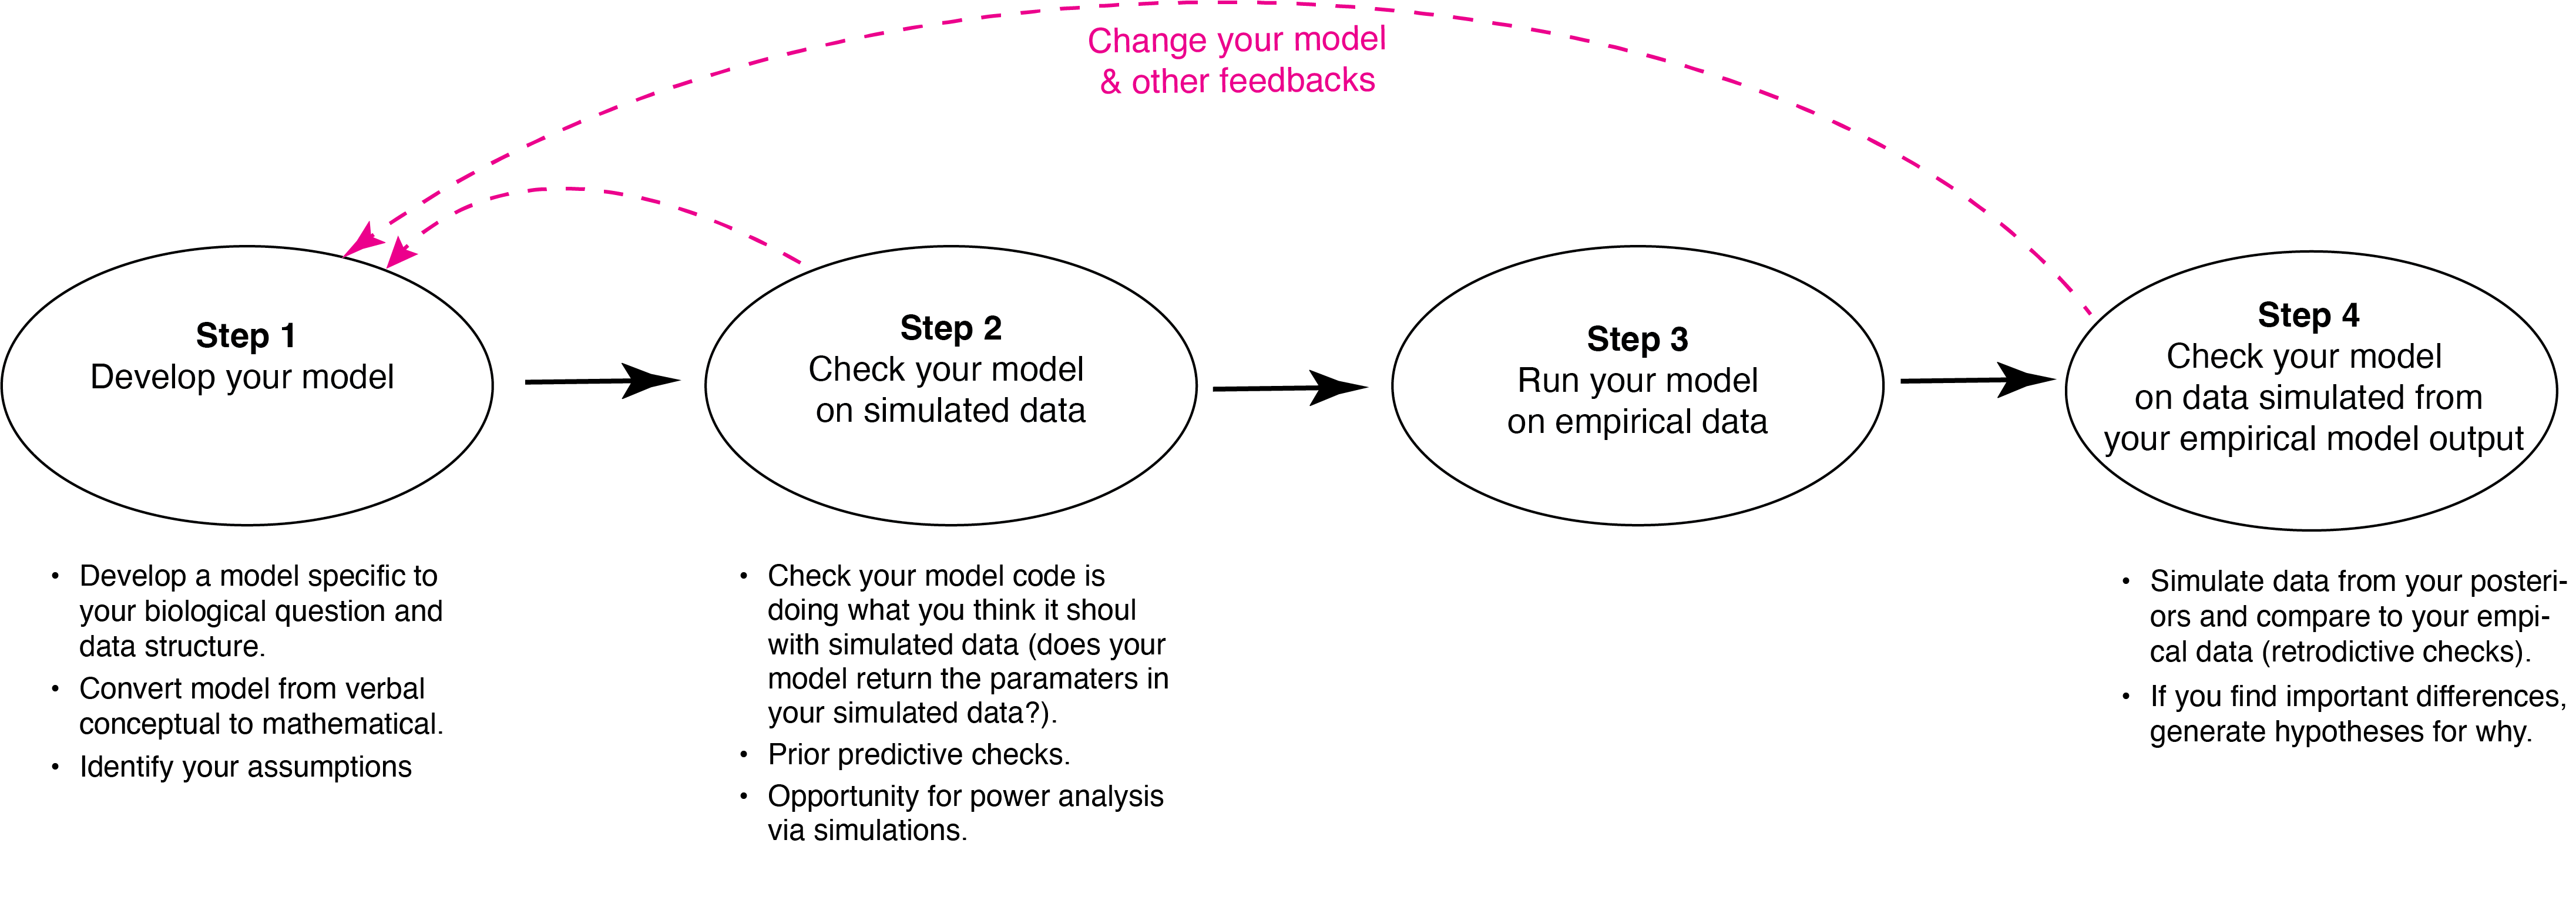
\includegraphics[width=1\textwidth]{figures/workflow.png}
\caption{The four-step iterative workflow we outline can help design models for specific ecological questions, data and aims---which makes this a statistical workflow that can naturally become a scientific workflow. It makes the step that many of us focus on---running your model on your empirical data (Step 3)---far more straightforward and insightful by using simulations both before (Step 2) and after (Step 4) it to better understand the model and data together.}
\label{fig:workflow}
\end{figure}

\begin{figure}[ht]
\centering
\noindent 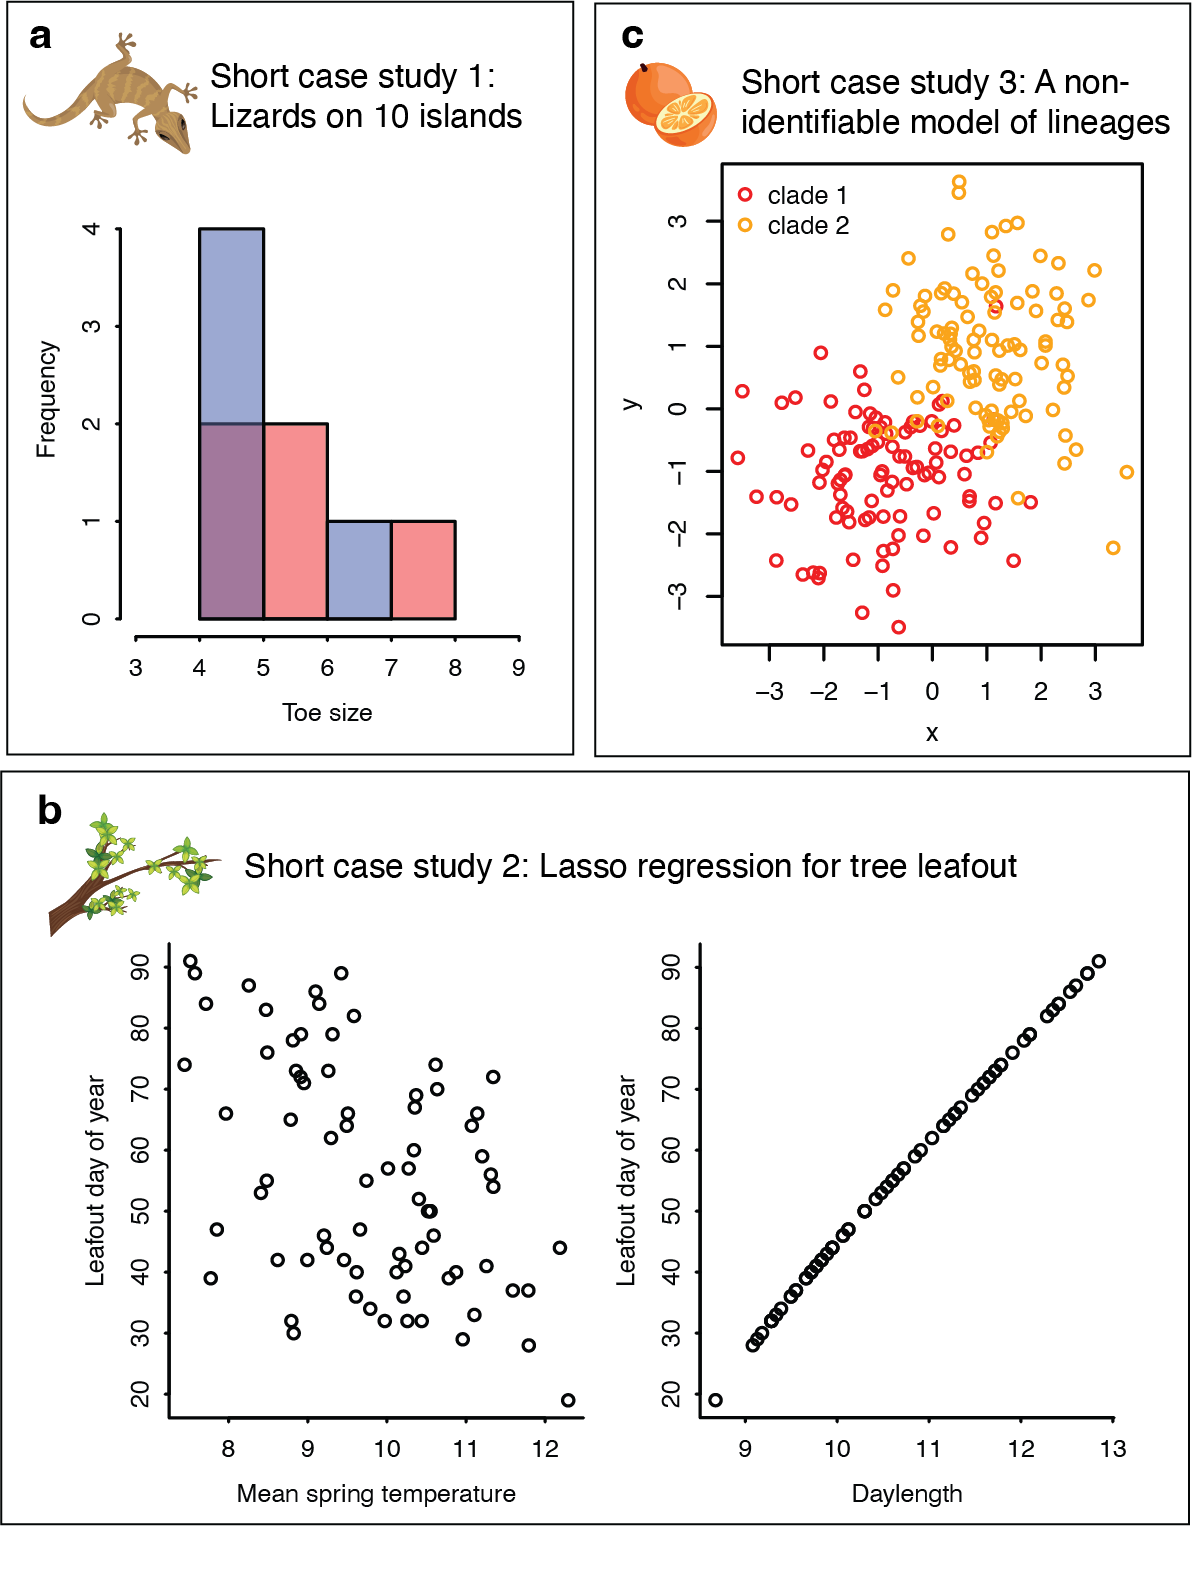
\includegraphics[width=0.8\textwidth]{figures/twoexamples.png}
\caption{We provide three very simple examples of the first steps of this workflow as Supplements (in PDF from R Markdown files). One example (a) uses ordinary least squares regression considering a natural experiment on lizards on tropical islands, and simulating two different possible sample sizes. The next example (b) uses lasso regression to examine how environmental variables may predict tree leafout. The third example (c) shows several examples of non-identifiability in regression models. See supplements: `Is a sample size of five stormy islands enough?'; `Identifying predictors of tree leafout' and `Three non-identifiable models, two of which are vital in biology.'}
\label{fig:twoexamples}
\end{figure}

\begin{figure}[ht]
\centering
\noindent 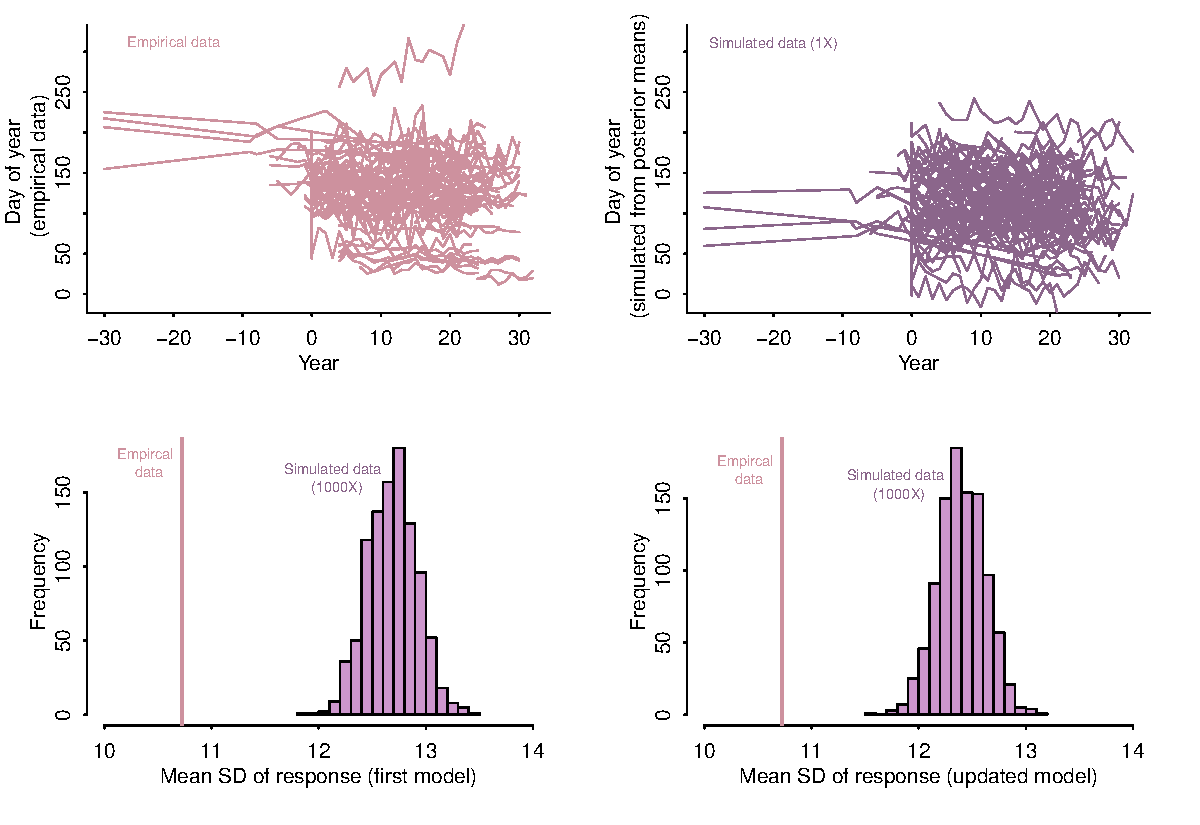
\includegraphics[width=0.95\textwidth]{examples/synchrony/graphs/fourpanelforpaper.pdf} % from 1000 sim. datasets (purple) \n versus empirical data (pink)
\caption{Example of retrodictive checks (Step 4) and feedbacks from time-series data of phenological events over time. The empirical data (top left, pink) looks similar to one simulated dataset (top right, purple), based on existing species number, their respective $x$ data, and simulating from the parameters for each species, but the spread of the simulated data seems possibly higher. Repeating this retrodictive (or posterior predictive) check 1000 times, and taking the standard deviation (SD) of each simulated dataset, then looking at the resulting histogram confirms this (lower left in purple, empirical data SD in pink). This leads to an updated model, where the same retrodictive check looks slightly closer to the empirical data (lower right), but clearly still could be improved as part of additional feedbacks. These examples are shown in full in `Steps 1-4 in a Bayesian framework' in the Supplement and available at: \url{https://github.com/lizzieinvancouver/bayesianflowsexample}.}
\label{fig:retrodictivecheck}
\end{figure}

\end{document}

